% Provenance (never printed): see sources/outline_sources.md (Year 1: solute and particle
% fluxes; the Hjulstrom diagram; settling velocity; denudation rates). Exercise and problem
% values in the Book 3 scratch calculator calc/ch20.py; figure data from
% figdata/bachelor-1/settling.py and threshold.py. Erosion, transport and deposition are
% Book 1's (g5); the sediment load in three forms, the denudation rate and isostatic rebound
% are Book 2's (g12), re-founded here (load, denudation rate) or recalled (rebound); discharge
% and the drainage basin are Book 2 g10's; Airy isostasy is ch. 11's; viscosity, Stokes' law
% and the Reynolds number are the physics books' (admitted, pointer). Grain-size classes and
% sorting belong to ch. 21.
\chapter{Erosión y transporte}\label{ch:b1:erosion-transport}

Tras una tormenta, el río bajo el puente baja de color marrón. El agua que el día anterior era clara está espesa de lodo, remolinea alrededor
de las pilas y arrastra ramas, y en el fondo, sin verse, los cantos rodados chocan entre sí al rodar. Cada segundo, la crecida se lleva toneladas
de tierra. Aguas abajo, tras una presa, ese mismo lodo se asienta en el agua quieta del embalse, que pierde un poco de volumen cada año; más lejos
aún, en la desembocadura del río, se extiende en el mar como una pluma parda que se puede ver desde el espacio. Este capítulo pone cifras a ese
viaje: cuánto transporta un río y en qué formas, con qué rapidez se hunde un grano, qué corriente necesita para ponerlo en movimiento, y con qué
rapidez, al fin, se desgasta un paisaje entero.

\begin{recall}
La erosión es el desgaste de la tierra y el arrastre de sus trozos; la sedimentación es su depósito allí donde el transportista se frena (libro 1,
año 5). Un río transporta su carga sedimentaria como \omterm{def:b1:erosion-transport:load}{carga de fondo}, \omterm{def:b1:erosion-transport:load}{carga en suspensión} y \omterm{def:b1:erosion-transport:load}{carga disuelta}; la \omterm{def:b1:erosion-transport:denudation}{tasa de denudación} de una región es
el espesor de roca que se le retira por unidad de tiempo, en metros por millón de años; cuando la erosión retira un espesor $e$ de \omterm{def:b1:layered-earth:layers}{corteza}, la
recuperación isostática solo deja bajar la superficie en $e(1 - \rho_c/\rho_m)$ (libro 2, año 12). El caudal de un río es el volumen de agua que pasa
por una sección transversal por unidad de tiempo, y su cuenca de drenaje el área que lo alimenta (libro 2, año 10). En la \omterm{prop:b1:isostasy-gravity:airy}{isostasia de Airy} la
\omterm{def:b1:layered-earth:layers}{corteza} flota sobre el \omterm{def:b1:layered-earth:layers}{manto} con una raíz proporcional a su relieve (\cref{prop:b1:isostasy-gravity:airy}). La \omterm{def:b1:weathering-clays:hydrolysis}{hidrólisis} de los silicatos envía iones
y sílice disuelta a los ríos (\cref{def:b1:weathering-clays:hydrolysis}). La viscosidad dinámica $\mu$ de un fluido mide su resistencia a la cizalla,
y la viscosidad cinemática es $\nu = \mu/\rho$; una esfera de diámetro $d$ que se mueve despacio a la velocidad $w$ a través de un fluido sufre el
arrastre $3\pi\mu d w$ (ley de Stokes); el número de Reynolds $w d/\nu$ compara la inercia con las fuerzas viscosas, y el flujo alrededor de la esfera es
suave mientras sea pequeño (libros de física).
\end{recall}

\section{Flujos de solutos y de partículas}\label{sec:b1:erosion-transport:fluxes}

Un río elimina la tierra de dos maneras: como materia en disolución, productos de la \omterm{def:b1:weathering-clays:weathering}{meteorización química}, y como granos sólidos, productos de la
\omterm{def:b1:weathering-clays:weathering}{meteorización física} y residuos insolubles de la \omterm{def:b1:weathering-clays:weathering}{meteorización química}. Los dos viajan de forma distinta, y los propios granos viajan de dos maneras.

\begin{definition}[Carga disuelta, carga en suspensión, carga de fondo]\label{def:b1:erosion-transport:load}
La carga de un río es la materia que transporta más allá de una sección transversal, en tres partes que se distinguen por cómo viajan. La
\emph{carga disuelta}\index{carga disuelta} es la materia en disolución, iones y sílice disuelta, que se mueve con el agua a su propia velocidad.
La \emph{carga en suspensión}\index{carga en suspensión} está formada por granos sostenidos dentro del flujo por su turbulencia, sobre todo arcilla,
limo y arena fina, que se mueven casi a la velocidad del agua y raramente tocan el fondo. La \emph{carga de fondo}\index{carga de fondo} está formada
por granos que ruedan, se deslizan o saltan a lo largo del fondo, en contacto frecuente con él, mucho más despacio que el agua.
\end{definition}

\begin{omfigure}
\begin{tikzpicture}[font=\footnotesize, >={Stealth[length=4pt]}]
% schematic: the three loads of a river (side view) and the forces on a bed grain
\fill[omDef!12] (0,0) rectangle (9,3.2);
\draw[omDef!80!black, thick] (0,3.2) -- (9,3.2);
\node[anchor=south west, omDef!80!black] at (0,3.2) {superficie del agua};
% flow profile arrows (velocity grows upward)
\foreach \y/\l in {0.35/0.5, 0.8/0.9, 1.4/1.15, 2.1/1.3, 2.8/1.4} {\draw[->, black!55] (0.25,\y) -- ++(\l,0);}
\draw[black!55] (0.25,0.12) -- (0.25,3.05);
\node[anchor=north west, black!65, align=left] at (0.2,-0.15) {perfil de\\ velocidad del flujo};
% bed
\fill[black!12] (0,-0.05) rectangle (9,0.12);
\foreach \x in {0.1,0.45,...,8.9} {\fill[black!45] (\x,0.0) circle[radius=0.09];}
% dissolved load: ions
\foreach \x/\y/\s in {2.3/2.7/+, 3.1/1.9/-, 4.0/2.85/+, 4.7/2.2/-, 5.6/2.75/+, 6.3/1.85/+, 7.2/2.6/-, 8.2/2.2/+, 2.7/1.2/-, 7.8/1.3/-} {\node[circle, draw=omThm, inner sep=0.2pt, minimum size=7pt, font=\tiny, text=omThm] at (\x,\y) {$\s$};}
% suspended load: fine grains, denser near the bed
\foreach \x/\y in {2.1/1.5, 2.6/0.9, 3.0/2.5, 3.4/0.6, 3.7/1.4, 4.2/0.8, 4.4/1.9, 4.9/0.55, 5.2/1.2, 5.5/2.1, 5.9/0.7, 6.1/1.5, 6.6/0.9, 6.9/2.3, 7.4/0.6, 7.6/1.7, 8.0/0.85, 8.5/1.4, 3.9/0.45, 5.0/0.35, 6.4/0.4, 2.4/0.45, 8.6/0.5} {\fill[brown!75!black] (\x,\y) circle[radius=0.05];}
% bed load: rolling and hopping grains
\fill[black!60] (3.2,0.27) circle[radius=0.15];
\draw[->, black!70] (3.0,0.55) arc[start angle=150, end angle=30, radius=0.25];
\fill[black!60] (5.6,0.25) circle[radius=0.12];
\draw[->, black!70, densely dashed] (4.6,0.2) .. controls (4.9,0.9) and (5.3,0.7) .. (5.55,0.4);
\fill[black!60] (4.6,0.22) circle[radius=0.06];
% labels
\node[omThm, anchor=west] at (9.2,2.5) {carga disuelta: iones};
\node[brown!75!black, anchor=west] at (9.2,1.5) {carga en suspensión:};
\node[brown!75!black, anchor=west] at (9.2,1.1) {arcilla, limo, arena fina};
\node[black!75, anchor=west] at (9.2,0.4) {carga de fondo: granos que};
\node[black!75, anchor=west] at (9.2,0.0) {ruedan, se deslizan, saltan};
\draw[->, thick, black!70] (6.8,3.55) -- node[above] {flujo} (8.6,3.55);
% inset: forces on a grain resting on two others; it pivots about its downstream contact
\begin{scope}[xshift=11.8cm, yshift=-2.2cm]
  \fill[black!12] (-1.2,-0.4) rectangle (1.2,0);
  \fill[black!40] (-0.6,-0.15) circle[radius=0.28]; \fill[black!40] (0.6,-0.15) circle[radius=0.28];
  \fill[black!65] (0,0.166) circle[radius=0.4];
  \draw[->, thick, omDef!80!black] (0,0.166) -- (0,1.15) node[above] {sustentación};
  \draw[->, thick, omThm] (0,0.166) -- (1.05,0.166) node[right] {arrastre};
  \draw[->, thick, black] (0,0.166) -- (0,-0.8) node[below] {peso sumergido};
  \draw[->, thick, black!60] (-1.4,0.85) -- (-0.5,0.85) node[pos=0, left] {flujo};
  \fill[red!60!black] (0.353,-0.020) circle[radius=0.045];
  \node[font=\scriptsize, anchor=north west, black!70] at (0.5,-0.4) {pivote};
\end{scope}
\end{tikzpicture}

{\small Las tres cargas de un río, vistas de lado (esquemático, sin escala). El flujo es más rápido cerca de la superficie y se frena hasta
cero en el fondo. Los iones están repartidos por toda la profundidad; los granos en suspensión son arrastrados por los remolinos, y más de ellos
cerca del fondo; los granos de la \omterm{def:b1:erosion-transport:load}{carga de fondo} ruedan, se deslizan o dan saltos cortos. A la derecha: las fuerzas sobre un grano del fondo. El
arrastre y la sustentación del flujo tienden a hacerlo rodar sobre su vecino de aguas abajo, alrededor del punto de contacto; su peso en el agua
lo retiene.}
\label{fig:b1:erosion-transport:loads}
\end{omfigure}

La frontera entre las dos cargas sólidas no la fija el tamaño del grano: depende del flujo. Una crecida que transporta arena en suspensión la deja
en el fondo, como \omterm{def:b1:erosion-transport:load}{carga de fondo}, cuando baja; la arcilla más fina, en cambio, permanece en suspensión en casi cualquier corriente y apenas se
encuentra en el fondo de un río que fluye. Cada carga se mide como un flujo, una masa por unidad de tiempo que atraviesa una sección transversal del río.

\begin{proposition}[Flujo de una carga]\label{prop:b1:erosion-transport:flux}
Sea $c$ la concentración de una \omterm{def:b1:erosion-transport:load}{carga disuelta} o en suspensión (masa por unidad de volumen de agua) y $u$ la velocidad del agua, ambas variables a
través de la sección de área $A$. (1)~El flujo instantáneo de la carga a través de la sección es
\[
  F = \iint_A c\,u\,\mathrm dA = \overline{c}_Q\,Q,
\]
donde $Q = \iint_A u\,\mathrm dA$ es el caudal y $\overline{c}_Q$ la concentración media ponderada por la velocidad. (2)~Durante un periodo $T$ en el que el
caudal $Q(t)$ y la concentración $C(t)$ del río varían, la masa transportada es
\[
  M = \int_0^T Q\,C\,\mathrm dt = T\left(\overline{Q}\;\overline{C} +
  \operatorname{cov}(Q, C)\right),
\]
donde las barras son medias temporales y $\operatorname{cov}(Q, C)$ es la media de
$(Q - \overline{Q})(C - \overline{C})$. El producto del caudal medio y la concentración media da la masa correcta solo si ambos no están correlacionados.
\end{proposition}

\begin{proof}
(1)~En un tiempo $\mathrm dt$, el agua que atraviesa un pequeño área $\mathrm dA$ de la sección llena un volumen $u\,\mathrm dA\,\mathrm dt$, que lleva la masa
$c\,u\,\mathrm dA\,\mathrm dt$; sumando sobre la sección se obtiene $F$, y $\overline{c}_Q$ se define como $F/Q$. (2)~Escríbase $Q = \overline{Q} + Q'$ y $C =
\overline{C} + C'$, donde las fluctuaciones $Q'$ y $C'$ tienen media nula en el periodo. Entonces $QC = \overline{Q}\,\overline{C} + \overline{Q}\,C' + Q'\,\overline{C}
+ Q'C'$; los dos términos del medio promedian cero, y la media de $Q'C'$ es la covarianza.
\end{proof}

La covarianza importa para la \omterm{def:b1:erosion-transport:load}{carga en suspensión}. Su concentración sube bruscamente en las crecidas, cuando la lluvia lava la tierra hacia los arroyos y
el flujo más rápido levanta granos del fondo, así que $Q$ y $C$ crecen juntos: una gran parte del sedimento anual de un río pasa en unos pocos días de
crecida, y una campaña de muestreo que los pierda, o una concentración media multiplicada por el caudal medio, subestima la carga. La \omterm{def:b1:erosion-transport:load}{carga disuelta} se
comporta al revés: las crecidas la diluyen, y su concentración es mayor en caudal bajo, cuando el río se alimenta de agua subterránea que ha estado mucho
tiempo en contacto con la roca.

\begin{method}[La carga anual de un río a partir de aforos]\label{met:b1:erosion-transport:gauging}
\begin{enumerate}
  \item Regístrese el caudal de forma continua en una estación de aforo.
  \item Muéstrese el agua con muchos caudales, las crecidas incluidas, y mídase la masa de sedimento por litro (filtrando y pesando) y la de cada
        especie disuelta.
  \item Pondérense las concentraciones por el caudal en el momento del muestreo para obtener la concentración media ponderada por el flujo, o ajústese
        la concentración como función del caudal y aplíquese a todo el registro.
  \item Multiplíquese por el volumen total de agua del año, o súmese $Q\,C\,\Delta
        t$ sobre el registro (\cref{prop:b1:erosion-transport:flux}).
  \item Añádase la \omterm{def:b1:erosion-transport:load}{carga de fondo}, que los muestreadores de agua no recogen, a partir de medidas separadas o como una fracción estimada.
  \item Para la \omterm{def:b1:erosion-transport:load}{carga disuelta}, quítese lo que no procede de la roca: las sales traídas por la lluvia y, para el bicarbonato, el carbono tomado del aire
        (\cref{ch:b1:weathering-clays}).
\end{enumerate}
\end{method}

\begin{omfigure}
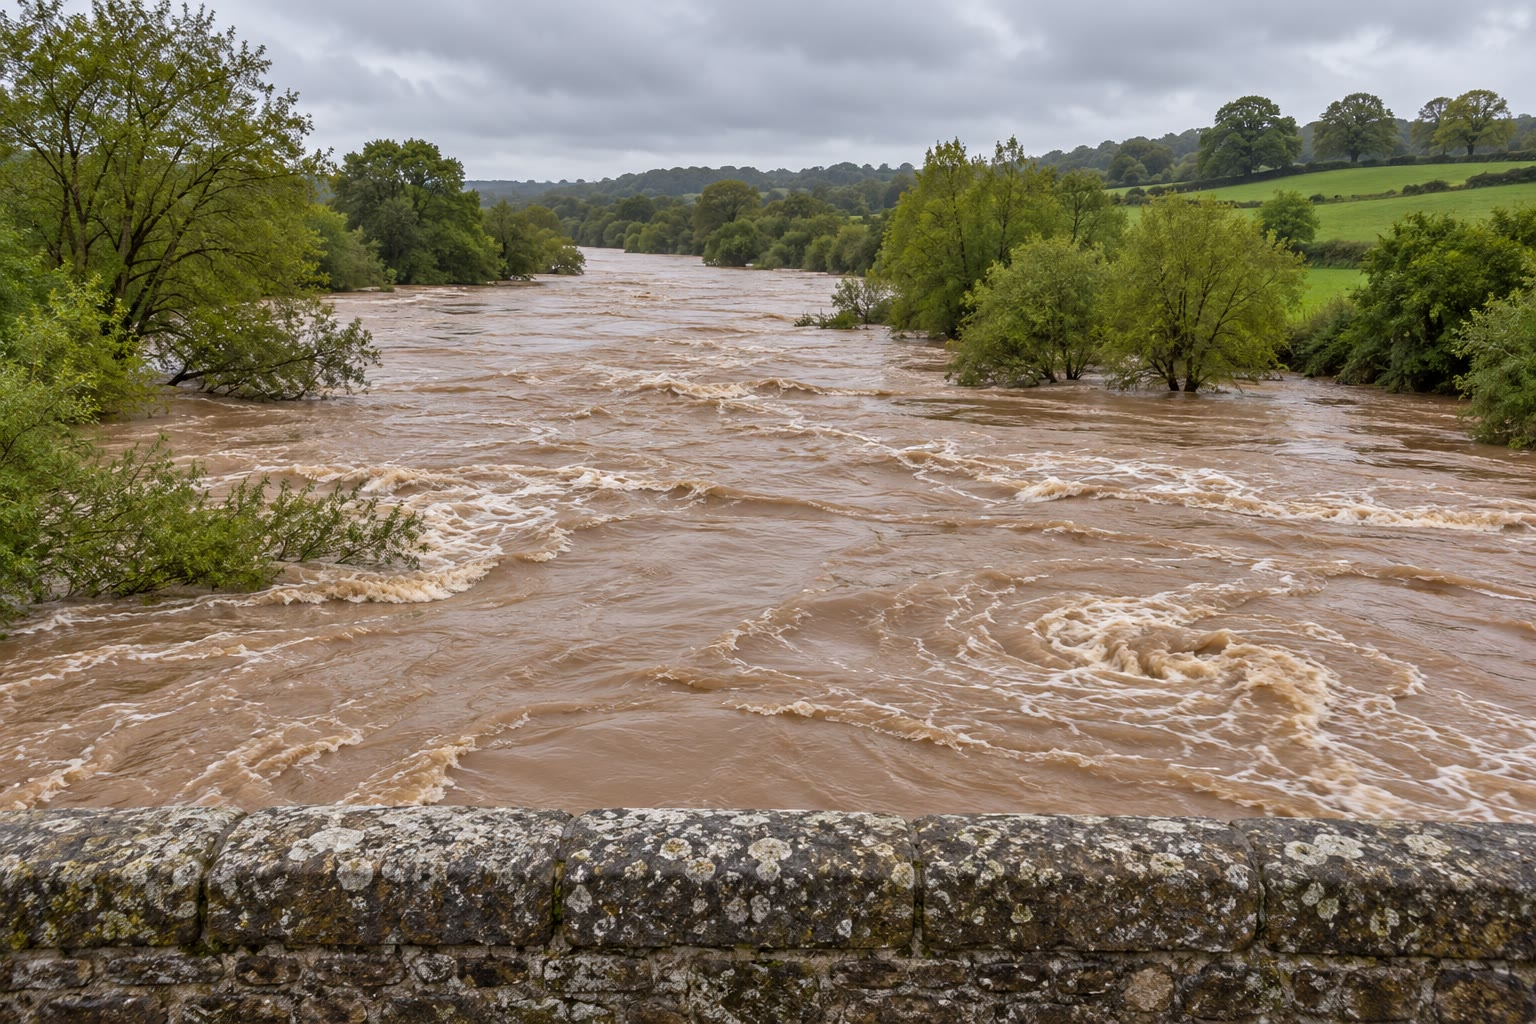
\includegraphics[height=5.1cm]{images/book3/ai/b1-muddy-river.jpg}\hfill
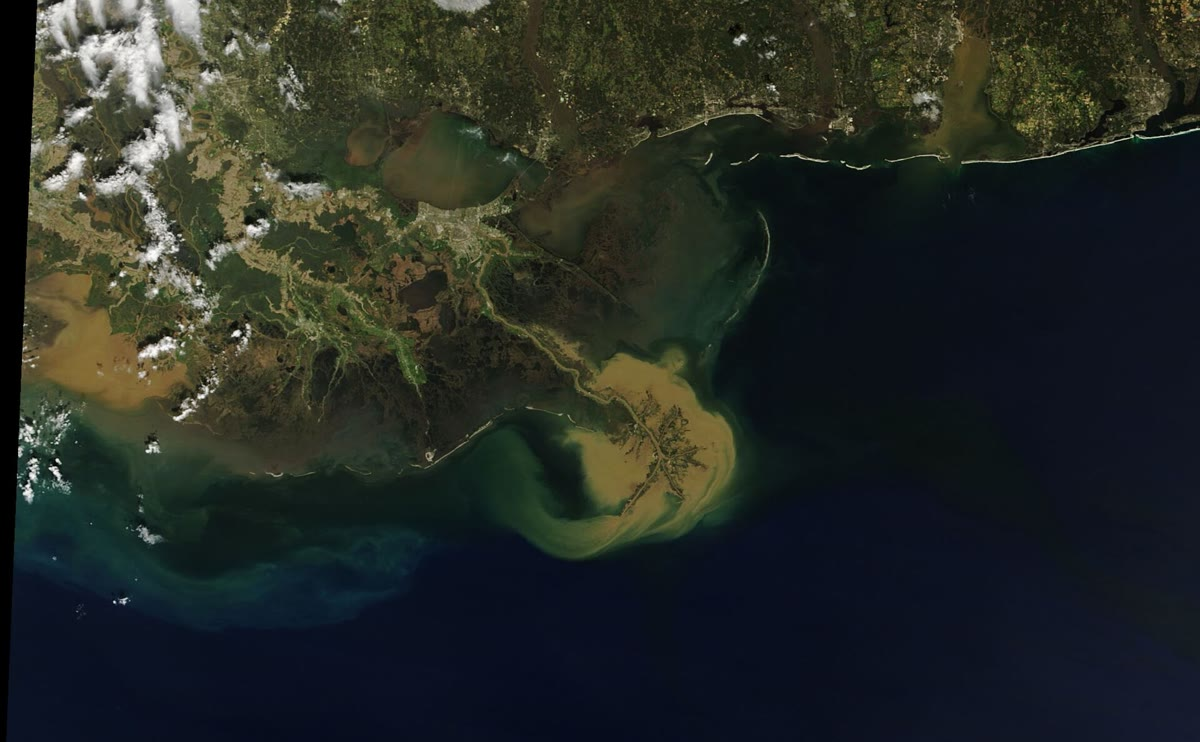
\includegraphics[height=5.1cm]{images/book3/b1-mississippi-plume.jpg}
\par\smallskip{\small Izquierda: un río en crecida lleva agua parda cargada de sedimento (ilustración IA). Derecha: la pluma de inundación del
Misisipi vertiéndose en el golfo de México alrededor de su delta, vista por el instrumento MODIS del satélite Terra el 4 de marzo de 2018; el lodo en
suspensión tiñe el mar de pardo y verde, y el viento del sudeste empuja la pluma hacia el noroeste. Imagen del Observatorio de la Tierra de la NASA
de Joshua Stevens, dominio público, a través de Wikimedia Commons.}
\label{fig:b1:erosion-transport:plume}
\end{omfigure}
% ledger: commons:mississippi-plume

\emph{Los ríos del mundo.} Antes de cualquier influencia humana, los ríos del mundo llevaban al océano costero unas \qty{14}{Gt} de sedimento en
suspensión al año, \qty{15.5}{Gt} con la \omterm{def:b1:erosion-transport:load}{carga de fondo}. Las personas han cambiado ambos extremos del viaje: la agricultura y la deforestación
han aumentado la erosión del suelo, añadiendo unas \qty{2.3}{Gt} al año a los ríos, mientras que los embalses retienen sedimento: los grandes
atrapan alrededor del \qty{20}{\percent} del flujo y los pequeños otro \qty{6}{\percent}, y más de \qty{100}{Gt} de sedimento yacen ahora detrás de
presas construidas sobre todo en los últimos cincuenta años. El efecto neto es una reducción: el flujo actual es de unos \qty{12.6}{Gt} al año.
% ledger: syvitski:flux

\begin{dated}{2005}
Las cifras del flujo de sedimento en suspensión, antes y después de la influencia humana, proceden de un modelo global del sedimento de los
ríos publicado en 2005. Desde entonces se han construido presas.
\end{dated}
% ledger: syvitski:flux

La \omterm{def:b1:erosion-transport:load}{carga disuelta} es menor. Una recopilación clásica de análisis de ríos, hecha en 1963, situó la materia disuelta que los ríos del mundo entregan al mar
en unas \qty{3.9}{Gt} al año, cerca del \qty{30}{\percent} del flujo actual en suspensión, con una concentración media de \qty{120}{mg} por litro.
El bicarbonato constituye casi la mitad, \qty{58}{mg.L^{-1}}, seguido del calcio, la sílice, el sulfato, el cloruro y el sodio. Parte de ella no procede
de la roca: buena parte del bicarbonato lleva carbono tomado del aire o del suelo, y parte del cloruro y del sodio procede de la sal marina arrastrada
por la lluvia. Los ríos individuales se separan mucho de estas medias.
% ledger: livingstone:world-dissolved, syvitski:flux

\emph{El presupuesto sedimentario de una cuenca.} No todo grano erosionado en una cuenca de drenaje llega a su desembocadura. La tierra arrastrada
desde un campo puede detenerse al pie de la ladera, la arena puede almacenarse durante siglos en la llanura de inundación y en las barras del río, y un
embalse puede retener la mayor parte de lo que le llega. La carga medida en la desembocadura es el saldo del presupuesto: lo que se erosiona en las laderas
y en las orillas, menos lo que se almacena en el camino, más lo que se recupera de viejos depósitos. En unas pocas décadas de aforos este saldo puede
diferir mucho de la tasa de erosión a largo plazo, en un sentido o en el otro, lo que es una razón para los otros métodos de
\cref{sec:b1:erosion-transport:denudation}.

\section{Velocidad de sedimentación}\label{sec:b1:erosion-transport:settling}

Un grano es más denso que el agua y se hunde. Si un río puede transportarlo, y dónde se depositará, depende ante todo de la rapidez con que se hunde.

\begin{definition}[Velocidad de sedimentación]\label{def:b1:erosion-transport:settling}
La \emph{velocidad de sedimentación}\index{velocidad de sedimentación} $w_s$ de un grano es la velocidad constante con la que cae a través de agua en reposo, cuando
el arrastre del agua equilibra su peso sumergido, es decir, su peso menos el empuje del agua que desaloja.
\end{definition}

Un grano liberado en agua quieta se acelera hasta que su arrastre, que crece con su velocidad, equilibra su peso sumergido; para un grano de arena o de limo esto
lleva una pequeña fracción de segundo, así que la \omterm{def:b1:erosion-transport:settling}{velocidad de sedimentación} es la velocidad a la que cae casi todo el trayecto. Con las densidades $\rho_s$
del grano y $\rho$ del agua, escríbase $R = (\rho_s - \rho)/\rho$ para la densidad sumergida relativa.

\begin{proposition}[Sedimentación de Stokes]\label{prop:b1:erosion-transport:stokes}
Una esfera de diámetro $d$ y densidad $\rho_s$ que cae despacio a través de agua de densidad $\rho$ y viscosidad dinámica $\mu$, según la ley de Stokes,
tiene la \omterm{def:b1:erosion-transport:settling}{velocidad de sedimentación}
\[
  w_s = \frac{(\rho_s - \rho)\,g\,d^2}{18\,\mu} = \frac{R\,g\,d^2}{18\,\nu}.
\]
La ley vale mientras el número de Reynolds del grano $w_s d/\nu$ esté por debajo de unos 1, es decir, para diámetros menores que
$d_1 = \left(18\,\nu^2/(R\,g)\right)^{1/3}$.
\end{proposition}

\begin{proof}
El peso de la esfera es $\rho_s g\,\pi d^3/6$ y el empuje $\rho g\,\pi d^3/6$, así que su peso sumergido es $(\rho_s - \rho)\,g\,\pi d^3/6$.
En la \omterm{def:b1:erosion-transport:settling}{velocidad de sedimentación} iguala al arrastre $3\pi\mu d\,w_s$:
\[
  (\rho_s - \rho)\,g\,\frac{\pi d^3}{6} = 3\pi\mu d\,w_s
  \quad\Longrightarrow\quad
  w_s = \frac{(\rho_s - \rho)\,g\,d^2}{18\,\mu},
\]
y dividiendo el numerador y el denominador por $\rho$ se obtiene la segunda forma. El número de Reynolds de esta velocidad es $R g d^3/(18\nu^2)$, que
vale 1 para $d = d_1$ y crece como $d^3$.
\end{proof}

Para el cuarzo, de densidad \qty{2650}{kg.m^{-3}}, en agua a \qty{20}{\celsius}, de densidad \qty{998.2}{kg.m^{-3}} y viscosidad \qty{1.0016}{mPa.s}:
$R =
1.65$, $\nu = \qty{1.003e-6}{m^2.s^{-1}}$, y con $g =
\qty{9.81}{m.s^{-2}}$ el límite es $d_1 = \qty{0.104}{mm}$, una arena fina. Por debajo, la ley de Stokes da las \omterm{def:b1:erosion-transport:settling}{velocidades de sedimentación} del limo y la arcilla: un grano de limo
de \qty{10}{\micro m} de diámetro se hunde a \qty{9.0e-5}{m.s^{-1}}, \qty{1}{m} en unas tres horas; una partícula de arcilla de \qty{2}{\micro m} a
\qty{3.6e-6}{m.s^{-1}}, \qty{1}{m} en \num{3.2}~días. Las partículas naturales de arcilla son escamas, no esferas, y se hunden aún más despacio. Agua de
\qty{5}{m} de profundidad, perfectamente quieta, tardaría dieciséis días en quedar libre de esa arcilla; un río que fluye, cuyos remolinos la mantienen
agitada, nunca lo consigue, y por eso el lodo más fino viaja hasta el mar.
% ledger: hom:quartz, nist:water, const:gn

Por encima de $d_1$ el arrastre crece más deprisa que en proporción a la velocidad: el agua que fluye junto al grano se separa tras él en una estela, y a
números de Reynolds grandes el arrastre es proporcional al cuadrado de la velocidad. Los experimentos con granos naturales se resumen en una sola fórmula que
une los dos regímenes.

\begin{proposition}[Ley combinada de sedimentación]\label{prop:b1:erosion-transport:combined}
La \omterm{def:b1:erosion-transport:settling}{velocidad de sedimentación} de granos naturales de diámetro de tamiz $d$ es, para todos los tamaños,
\[
  w_s = \frac{R\,g\,d^2}{C_1\,\nu + \sqrt{0.75\,C_2\,R\,g\,d^3}},
\]
con $C_1 = 18$ y $C_2 = 1.0$.
\end{proposition}
\admitted
% ledger: fc:settling

La ley se debe a Ferguson y Church, que la ajustaron a \omterm{def:b1:erosion-transport:settling}{velocidades de sedimentación} medidas en arenas naturales. Para granos pequeños la raíz cuadrada es
despreciable y se reduce a la ley de Stokes; para granos grandes el primer término del denominador es despreciable y $w_s \to \sqrt{4 R g d/(3 C_2)}$, que
crece solo como la raíz cuadrada del tamaño. Las constantes dependen de la forma de los granos: $C_2 = 0.4$ describe esferas lisas, y valores mayores granos
más angulosos, que encuentran más arrastre. Las dos leyes se separan por encima de \qty{0.1}{mm}. Para un grano de \qty{1}{mm} la ley combinada da
\qty{0.126}{m.s^{-1}}, siete veces menos que la ley de Stokes; para un canto de \qty{10}{mm}, \qty{0.46}{m.s^{-1}} frente a los \qty{90}{m.s^{-1}} sin sentido
de la ley de Stokes (diagrama de abajo).
% ledger: fc:settling

\begin{omfigure}
\begin{tikzpicture}[font=\small]
% settling velocity of quartz grains in water at 20 C (figdata/bachelor-1/settling.py)
\begin{axis}[width=11cm, xmode=log, ymode=log, xmin=0.001, xmax=10, ymin=1e-8, ymax=10, height=8cm,
  xlabel={diámetro del grano $d$ (\si{mm})}, ylabel={velocidad de sedimentación (\si{m.s^{-1}})},
    ytick={1e-8,1e-6,1e-4,1e-2,1},
    legend style={at={(0.03,0.97)}, anchor=north west, font=\footnotesize}, legend cell align=left,
    grid=major, grid style={black!10}]
  \addplot[omDef, thick, dashed] table[x=d_mm, y=w_stokes] {figdata/out/bachelor-1-settling-curves.dat};
  \addplot[omThm, very thick] table[x=d_mm, y=w_fc] {figdata/out/bachelor-1-settling-curves.dat};
  \legend{ley de Stokes, ley combinada (granos naturales)}
  \draw[black!55, densely dotted] (axis cs:0.1037,1e-7) -- (axis cs:0.1037,10);
  \node[font=\scriptsize, anchor=west, align=left, black!75] at (axis cs:0.115,1e-6) {número de Reynolds\\ del grano $= 1$};
  \node[font=\scriptsize, black!70] at (axis cs:0.002,3e-8) {arcilla};
  \node[font=\scriptsize, black!70] at (axis cs:0.016,3e-8) {limo};
  \node[font=\scriptsize, black!70] at (axis cs:0.35,3e-8) {arena};
  \node[font=\scriptsize, black!70] at (axis cs:4.5,3e-8) {grava};
  \draw[black!40] (axis cs:0.0039,1e-8) -- (axis cs:0.0039,1e-7);
  \draw[black!40] (axis cs:0.0625,1e-8) -- (axis cs:0.0625,1e-7);
  \draw[black!40] (axis cs:2,1e-8) -- (axis cs:2,1e-7);
\end{axis}
\end{tikzpicture}

{\small \omterm{def:b1:erosion-transport:settling}{Velocidad de sedimentación} de granos de cuarzo en agua a \qty{20}{\celsius}, frente a su diámetro, ambos en escalas logarítmicas: la ley de
Stokes y la ley combinada de los granos naturales, calculadas. En estas escalas la ley de Stokes es una recta de pendiente 2. Las dos coinciden para el
limo y la arcilla; por encima de unos \qty{0.1}{mm}, donde el número de Reynolds del grano pasa de 1, el arrastre de la estela frena los granos gruesos.
Las marcas de la parte inferior señalan los límites de las clases granulométricas, en \qty{3.9}{\micro m} ($1/256$~mm), \qty{62.5}{\micro m}
($1/16$~mm) y \qty{2}{mm}.}
\label{fig:b1:erosion-transport:settling}
\end{omfigure}
% ledger: fc:settling, usgs:wentworth-phi

En todo el intervalo del diagrama, desde la arcilla más fina hasta una grava gruesa, la \omterm{def:b1:erosion-transport:settling}{velocidad de sedimentación} abarca ocho órdenes de magnitud.
Esta es la primera razón por la que los ríos clasifican su sedimento: una corriente que se frena deja caer su grava de inmediato, su arena a metros,
su limo a kilómetros, y lleva su arcilla a un lago o al mar. Las clases granulométricas y la clasificación de los sedimentos son el tema del capítulo
siguiente (\cref{ch:b1:clastic-sediments}).

\section{Umbral de movimiento y diagrama de Hjulström}\label{sec:b1:erosion-transport:threshold}

Un grano en reposo en el fondo de un río es puesto en movimiento por la fuerza del agua que fluye sobre él. Esa fuerza se mide con un esfuerzo.

\begin{definition}[Esfuerzo de cizalla en el fondo, velocidad de cizalla]\label{def:b1:erosion-transport:bed-shear}
El \emph{esfuerzo de cizalla en el fondo}\index{esfuerzo de cizalla en el fondo} $\tau_b$ de un flujo es la fuerza por unidad de área que ejerce sobre
su fondo, paralela al fondo, en el sentido del flujo. La velocidad de cizalla es $u_* = \sqrt{\tau_b/\rho}$, una velocidad que mide el mismo esfuerzo.
\end{definition}

El \omterm{def:b1:erosion-transport:bed-shear}{esfuerzo de cizalla en el fondo} no puede leerse en un medidor de corriente, pero en un flujo estacionario se deduce de un equilibrio de fuerzas.

\begin{proposition}[Producto profundidad--pendiente]\label{prop:b1:erosion-transport:depth-slope}
En un flujo estacionario y uniforme de profundidad $h$ por un canal ancho de pendiente pequeña $S$, el \omterm{def:b1:erosion-transport:bed-shear}{esfuerzo de cizalla en el fondo} es
\[
  \tau_b = \rho\,g\,h\,S .
\]
\end{proposition}

\begin{proof}
Considérese el agua sobre un trozo de fondo de longitud $L$ a lo largo del flujo y de anchura unitaria, siendo el canal tan ancho que sus orillas
pueden ignorarse. El flujo es estacionario y uniforme, así que esta agua no se acelera y las fuerzas sobre ella se equilibran. Las fuerzas de presión
sobre sus caras aguas arriba y aguas abajo son iguales y opuestas, pues la profundidad es la misma en ambas. A lo largo del flujo quedan la componente
del peso, $\rho g h L \sin\beta$, donde $\beta$ es el ángulo del fondo, y el rozamiento del fondo, $\tau_b L$, que se le opone. Por tanto $\tau_b
= \rho g h \sin\beta$, y para un ángulo pequeño $\sin\beta \approx \tan\beta = S$.
\end{proof}

Un río de \qty{2}{m} de profundidad con una pendiente de \num{0.001}, un metro de desnivel por kilómetro, tiene $\tau_b = 998.2 \times 9.81 \times 2 \times 0.001 =
\qty{19.6}{Pa}$, y una velocidad de cizalla de \qty{0.140}{m.s^{-1}}. En un canal que no es ancho, las orillas toman su parte del rozamiento, y la
profundidad se sustituye por el radio hidráulico, el área de la sección dividida por su perímetro mojado (\cref{exo:b1:erosion-transport:5}).

\emph{Fuerzas sobre un grano.} El flujo empuja un grano del fondo con su arrastre, y lo levanta con el flujo más rápido sobre su cima (el recuadro
de la primera figura de este capítulo). Ambas fuerzas actúan sobre el área del grano, así que escalan como $\tau_b
d^2$; el grano resiste con su peso sumergido, que escala como
$(\rho_s - \rho) g d^3$. El cociente de ambas es la medida natural de la intensidad del flujo para un grano dado.

\begin{definition}[Parámetro de Shields, umbral de movimiento]\label{def:b1:erosion-transport:threshold}
El \emph{parámetro de Shields}\index{parámetro de Shields} de un flujo de \omterm{def:b1:erosion-transport:bed-shear}{esfuerzo de cizalla en el fondo} $\tau_b$ sobre granos de diámetro $d$ y densidad $\rho_s$ es
\[
  \theta = \frac{\tau_b}{(\rho_s - \rho)\,g\,d}.
\]
El \emph{umbral de movimiento}\index{umbral de movimiento} de los granos es el \omterm{def:b1:erosion-transport:bed-shear}{esfuerzo de cizalla en el fondo}, o el valor $\theta_c$ del parámetro de Shields,
al que empiezan a moverse.
\end{definition}
% ledger: hecras:thresholds

El valor crítico $\theta_c$ se mide en canales, y las medidas caen sobre una sola curva cuando se representan frente a un tamaño de grano adimensional que combina el grano y el fluido.

\begin{proposition}[Curva de umbral de Soulsby y Whitehouse]\label{prop:b1:erosion-transport:soulsby}
Para granos de diámetro $d$ sobre un fondo plano, con
$D_* = d\,\left(R\,g/\nu^2\right)^{1/3}$, el \omterm{def:b1:erosion-transport:threshold}{parámetro de Shields} crítico es
\[
  \theta_c = \frac{0.3}{1 + 1.2\,D_*} + 0.055\left(1 - e^{-0.02\,D_*}\right),
\]
y el esfuerzo de cizalla crítico en el fondo es $\tau_c = \theta_c\,(\rho_s - \rho)\,g\,d$.
\end{proposition}
\admitted
% ledger: hecras:thresholds

Para granos gruesos $\theta_c$ tiende a \num{0.055}: la grava se mueve cuando el \omterm{def:b1:erosion-transport:bed-shear}{esfuerzo de cizalla en el fondo} alcanza alrededor de una vigésima
parte del peso sumergido de una capa de granos de un diámetro de espesor, por unidad de área. Las fórmulas de transporte de sedimento que usan un
umbral constante toman valores de \num{0.03} a \num{0.047}, siendo este último el de la fórmula clásica de \omterm{def:b1:erosion-transport:load}{carga de fondo} de Meyer-Peter y Müller.
Para la arena fina $\theta_c$ vuelve a subir, hasta \num{0.077} a \qty{0.1}{mm}: los granos pequeños quedan dentro de la capa lenta y viscosa del agua
junto al fondo y están protegidos por sus vecinos. El mínimo, \num{0.030}, cae cerca de \qty{0.7}{mm}. En pascales el umbral crece siempre con el tamaño
(diagrama de abajo): \qty{0.13}{Pa} para una arena de \qty{0.1}{mm}, \qty{0.51}{Pa} a \qty{1}{mm}, \qty{9.0}{Pa} a \qty{10}{mm}, \qty{57}{Pa} para un
canto de \qty{64}{mm}.
% ledger: hecras:thresholds

\begin{omfigure}
\begin{tikzpicture}[font=\small]
% threshold of motion of quartz grains in water at 20 C (figdata/bachelor-1/threshold.py, Soulsby and Whitehouse)
\begin{axis}[name=a, width=6.9cm, height=6cm, xmode=log, xmin=0.0625, xmax=100, ymin=0, ymax=0.12,
xlabel={diámetro del grano $d$ (\si{mm})}, ylabel={parámetro de Shields crítico $\theta_c$},
    yticklabel style={/pgf/number format/fixed, /pgf/number format/precision=2},
    grid=major, grid style={black!10}, title={\footnotesize (a) adimensional}]
  \addplot[omThm, very thick] table[x=d_mm, y=theta] {figdata/out/bachelor-1-threshold-shields.dat};
  \draw[black!50, dashed] (axis cs:0.0625,0.055) -- (axis cs:100,0.055) node[pos=0.7, above, font=\scriptsize, black!70] {$0.055$};
\end{axis}
\begin{axis}[at={(a.east)}, anchor=west, xshift=2.0cm, width=6.9cm, height=6cm, xmode=log, ymode=log,
    xmin=0.0625, xmax=100, ymin=0.05, ymax=200,
    xlabel={diámetro del grano $d$ (\si{mm})}, ylabel={esfuerzo de cizalla crítico en el fondo $\tau_c$ (\si{Pa})},
    grid=major, grid style={black!10}, title={\footnotesize (b) en pascales}]
  \addplot[omDef, very thick] table[x=d_mm, y=tau_cr] {figdata/out/bachelor-1-threshold-shields.dat};
\end{axis}
\end{tikzpicture}

{\small El \omterm{def:b1:erosion-transport:threshold}{umbral de movimiento} de los granos de cuarzo en agua a \qty{20}{\celsius}, según la curva de Soulsby y Whitehouse, calculado desde el límite de
la arena fina (\qty{0.0625}{mm}) hasta el tamaño de un canto. (a)~El \omterm{def:b1:erosion-transport:threshold}{parámetro de Shields} crítico es casi constante para la grava y sube para la arena
fina. (b)~El esfuerzo de cizalla crítico en el fondo crece casi en proporción al diámetro para la grava.}
\label{fig:b1:erosion-transport:threshold}
\end{omfigure}
% ledger: hecras:thresholds

\begin{example}[Lo que mueve el río]\label{ex:b1:erosion-transport:river}
En el río de \qty{2}{m} de profundidad con pendiente de \num{0.001}, $\tau_b =
\qty{19.6}{Pa}$. Para granos de \qty{20}{mm}, $\theta = 19.6/(1651.8 \times
9.81 \times 0.020) = 0.060$, justo por encima de su umbral de \num{0.055}: se mueven. Para granos de \qty{40}{mm}, $\theta = 0.030$, la mitad del umbral:
se quedan. El río mueve su fondo hasta la grava gruesa; para la arena de \qty{1}{mm}, $\theta = 1.21$, casi cuarenta veces el umbral de \num{0.031}.
\end{example}

\emph{Hacia la suspensión.} Una vez en movimiento, un grano salta a lo largo del fondo o es recogido por el flujo, según si los remolinos, cuyas velocidades son
del orden de la velocidad de cizalla, pueden sostenerlo frente a su sedimentación.

\begin{proposition}[Criterio de suspensión]\label{prop:b1:erosion-transport:suspension}
Un grano de \omterm{def:b1:erosion-transport:settling}{velocidad de sedimentación} $w_s$ puede permanecer en suspensión en un flujo turbulento solo si algunos remolinos ascienden más deprisa de lo que
él se hunde. Como las velocidades ascendentes de los remolinos son del orden de la velocidad de cizalla $u_*$, la suspensión empieza cuando $u_*$ se acerca a $w_s$
y está plenamente desarrollada cuando $u_*$ la supera; este capítulo toma $u_* = w_s$ como límite de la suspensión.
\end{proposition}
\admitted
% ledger: bagnold:suspension

En el río del ejemplo, $u_* = \qty{0.140}{m.s^{-1}}$, que la ley combinada de sedimentación asigna a granos de \qty{1.16}{mm}: la arena más fina que
aproximadamente un milímetro viaja en suspensión, y la arena más gruesa y la grava como \omterm{def:b1:erosion-transport:load}{carga de fondo}. El argumento se remonta a Bagnold, que observó que
los granos de \qty{0.1}{mm} o menos quedan totalmente en suspensión en cuanto se mueven, mientras que los granos mayores de \qty{1}{mm} necesitan un \omterm{def:b1:erosion-transport:bed-shear}{esfuerzo de
cizalla en el fondo} muchas veces mayor que su umbral. Cuando la crecida baja y $u_*$ disminuye, la arena gruesa cae primero al fondo.

\emph{Del esfuerzo a la velocidad media.} Lo que se mide o se estima con facilidad en un río es su velocidad media. En un flujo turbulento sobre un fondo rugoso
por granos de diámetro $d$, un canal ancho de profundidad $h$ tiene la velocidad media
$U = u_*\left(6.25 + 5.75\log_{10}(h/d)\right)$, una ley establecida por Keulegan en 1938 a partir de los experimentos de Nikuradse y Bazin, así que el \omterm{def:b1:erosion-transport:threshold}{umbral de
movimiento} corresponde a la velocidad media crítica
\[
  U_c = \left(6.25 + 5.75\,\log_{10}\frac{h}{d}\right)\sqrt{\theta_c\,R\,g\,d},
\]
y el límite de suspensión, $u_* = w_s$, a $U_s = \left(6.25 +
5.75\log_{10}(h/d)\right) w_s$. Ambos dependen de la profundidad, aunque solo a través de un logaritmo.
% ledger: keulegan:mean-velocity, bagnold:suspension

Las velocidades de umbral pertenecen, pues, a una profundidad y a un conjunto de leyes: calculadas para otra profundidad, o leídas de otras mediciones, salen
distintas. Representadas frente al tamaño del grano, su forma es robusta pero sus valores no lo son, y el \omterm{def:b1:erosion-transport:bed-shear}{esfuerzo de cizalla en el fondo}, que no depende de la
profundidad de la misma manera, es la mejor medida de lo que puede hacer un flujo. Las velocidades siguen siendo más intuitivas, y la manera clásica de
dibujarlas es un diagrama.

\begin{definition}[Diagrama de Hjulström]\label{def:b1:erosion-transport:hjulstrom}
Un \emph{diagrama de Hjulström}\index{diagrama de Hjulström} representa la velocidad media de un flujo frente al diámetro de los granos, en escalas logarítmicas,
y divide el plano en los campos en que los granos en reposo son erosionados, los granos ya en movimiento se mantienen en transporte y los granos en movimiento
se depositan.
\end{definition}
% ledger: hjulstrom:curve

\begin{omfigure}
\begin{tikzpicture}[font=\small]
% Hjulstrom-type diagram for a flow 1 m deep (figdata/bachelor-1/threshold.py); the hatched
% cohesive field is schematic (its lower edge, 30 cm/s, is not computed)
\begin{axis}[width=12cm, height=8.4cm, xmode=log, ymode=log, xmin=0.001, xmax=100, ymin=0.1, ymax=3000,
  xlabel={diámetro del grano $d$ (\si{mm})}, ylabel={velocidad media del flujo (\si{cm.s^{-1}})},
    unbounded coords=jump, grid=major, grid style={black!10}]
  \addplot[draw=none, name path=dep] table[x=d_mm, y=u_dep] {figdata/out/bachelor-1-threshold-hjul.dat};
  \addplot[draw=none, name path=bot] coordinates {(0.001,0.1) (100,0.1)};
  \addplot[fill=omDef!14, draw=none] fill between[of=dep and bot];
  \fill[pattern=north east lines, pattern color=omThm!45] (axis cs:0.001,30) rectangle (axis cs:0.0625,3000);
  \addplot[omThm, very thick] table[x=d_mm, y=u_cr] {figdata/out/bachelor-1-threshold-hjul.dat};
  \addplot[omDef, very thick, dashed] table[x=d_mm, y=u_s] {figdata/out/bachelor-1-threshold-hjul.dat};
  \node[font=\footnotesize, fill=white, fill opacity=0.85, text opacity=1, align=center] at (axis cs:0.5,1500) {\textbf{erosión}: granos arrastrados en suspensión};
  \node[font=\footnotesize, fill=white, fill opacity=0.85, text opacity=1, align=center] at (axis cs:22,330) {\textbf{carga de fondo}};
  \node[font=\footnotesize, fill=white, fill opacity=0.85, text opacity=1, align=center] at (axis cs:0.0042,2.5) {\textbf{transporte}:\\ los granos ya\\ en movimiento\\ siguen en suspensión};
  \node[font=\footnotesize, fill=white, fill opacity=0.85, text opacity=1, align=center] at (axis cs:3,0.6) {\textbf{sedimentación}};
  \node[font=\footnotesize, fill=white, fill opacity=0.85, text opacity=1, align=center] at (axis cs:0.008,300) {lodo cohesivo:\\ umbral fijado por\\ la compactación};
  \node[font=\scriptsize, omThm, anchor=north, rotate=12] at (axis cs:6,80) {umbral de movimiento};
  \node[font=\scriptsize, omDef, anchor=north west, rotate=57] at (axis cs:0.028,0.95) {límite de suspensión};
  \draw (rel axis cs:0,0) -- (rel axis cs:1,0);
\end{axis}
\end{tikzpicture}

{\small Un diagrama de tipo Hjulström para granos de cuarzo en agua de \qty{1}{m} de profundidad a \qty{20}{\celsius}, calculado: el \omterm{def:b1:erosion-transport:threshold}{umbral de movimiento}
(sólido) según la curva de Soulsby y Whitehouse, el límite de suspensión (discontinuo) según la ley combinada de sedimentación, ambos convertidos en velocidades
medias mediante la ley de Keulegan. Por encima de la curva sólida, los granos en reposo son erosionados; por debajo de la menor de las dos curvas (sombreada),
los granos en movimiento se depositan. Los granos más finos que \qty{0.13}{mm} pasan a suspensión en cuanto se mueven; los más gruesos viajan primero como \omterm{def:b1:erosion-transport:load}{carga
de fondo}. El cálculo solo vale para granos sueltos: el campo rayado del limo y la arcilla cohesivos es esquemático.}
\label{fig:b1:erosion-transport:hjulstrom}
\end{omfigure}
% ledger: hecras:thresholds, fc:settling, bagnold:suspension, keulegan:mean-velocity

\emph{Lectura del diagrama.} Tres rasgos llevan la geología. Primero, los granos más fáciles de erosionar son las arenas finas, entre unos \num{0.06} y
\qty{0.2}{mm}, que una corriente de \qtyrange{31}{34}{cm.s^{-1}} pone en movimiento en agua de \qty{1}{m} de profundidad; los granos más gruesos necesitan más,
hasta unos \qty{3}{m.s^{-1}} para un canto de \qty{64}{mm}. Segundo, el limo y la arcilla, aunque son más ligeros, son más difíciles de erosionar que la arena
fina una vez asentados: sus partículas se pegan entre sí, y un lodo compactado resiste una corriente que arrastraría la arena. El cálculo para granos sueltos no
puede verlo, y las velocidades de erosión medidas de los lodos varían con su compactación y su contenido de agua, de ahí el campo rayado. Tercero, la brecha entre
erosión y sedimentación se abre mucho para los granos finos: una partícula de arcilla necesita una corriente fuerte para desprenderse de un fondo fangoso, pero una
vez en el agua permanece allí incluso en el flujo más suave, que es toda la historia de la crecida parda y de la pluma en el mar.
% ledger: hjulstrom:curve, hecras:thresholds, keulegan:mean-velocity

\begin{history}[Dos estudios de los años treinta]
En 1935 Filip Hjulström, del Instituto Geográfico de Uppsala, publicó un largo estudio de la obra del río Fyris, en el centro de Suecia, que contenía
el diagrama que lleva su nombre: velocidades de erosión y de sedimentación frente al tamaño del grano, en escalas logarítmicas. A diferencia de las
curvas anteriores, su curva de erosión tenía un mínimo, entre unos \num{0.1} y \qty{0.5}{mm}: la arena fina suelta es la más fácil de erosionar, mientras
que la arena más gruesa y la grava, y también el limo y la arcilla, que se cohesionan, necesitan corrientes más fuertes. Un año después, en 1936, el ingeniero
A.~Shields, en la tesis que defendió en la Escuela Técnica Superior de Berlín, representó el \omterm{def:b1:erosion-transport:threshold}{umbral de movimiento} como un cociente de fuerzas, el parámetro que
hoy lleva su nombre, frente a un tamaño de grano adimensional. Las velocidades de Hjulström ignoran la profundidad del flujo; el enfoque adimensional de Shields
no, y es la base de las fórmulas de umbral que se usan hoy, como la que está detrás de los diagramas de este capítulo.
\end{history}
% ledger: hjulstrom:curve, shields:1936, hecras:thresholds

\section{Tasas de denudación}\label{sec:b1:erosion-transport:denudation}

Las cargas de un río, sumadas sobre su cuenca, miden la rapidez con que la cuenca se desgasta.

\begin{definition}[Tasa de denudación]\label{def:b1:erosion-transport:denudation}
La \emph{tasa de denudación}\index{tasa de denudación} $D$ de una región es la velocidad media con que la retirada de materia, como granos sólidos y en
disolución, baja su superficie, expresada como el espesor equivalente de roca fresca por unidad de tiempo, en metros por millón de años (\unit{m/Myr}, lo mismo que
milímetros por mil años). La masa retirada por unidad de área y de tiempo, en toneladas por kilómetro cuadrado y por año, es el rendimiento específico de sedimento.
\end{definition}

\begin{proposition}[Denudación a partir de las cargas de los ríos]\label{prop:b1:erosion-transport:denudation}
Si una cuenca de área $A$ pierde, a través de su desembocadura, las masas anuales $F_s$ de \omterm{def:b1:erosion-transport:load}{carga en suspensión}, $F_b$ de \omterm{def:b1:erosion-transport:load}{carga de fondo} y $F_d$ de \omterm{def:b1:erosion-transport:load}{carga
disuelta} procedentes de sus rocas, y si no se almacena nada en el camino, su \omterm{def:b1:erosion-transport:denudation}{tasa de denudación} es
\[
  D = \frac{F_s + F_b + F_d}{\rho_r\,A},
\]
con $\rho_r$ la densidad de la roca fresca. Para $\rho_r =
\qty{2700}{kg.m^{-3}}$, un rendimiento específico de \qty{100}{t.km^{-2}.yr^{-1}} corresponde a \qty{37}{m/Myr}.
\end{proposition}

\begin{proof}
La masa perdida por unidad de área y de tiempo es $(F_s + F_b + F_d)/A$; dividida por la densidad de la roca se convierte en el espesor de roca perdido por
unidad de tiempo. Para la conversión, \qty{100}{t.km^{-2}.yr^{-1}} es
$\qty{1e5}{kg}/\qty{1e6}{m^2} = \qty{0.1}{kg.m^{-2}}$ al año, o
$0.1/2700 = \qty{3.7e-5}{m}$ al año, \qty{37}{m} por millón de años.
\end{proof}

La \omterm{def:b1:erosion-transport:load}{carga disuelta} cuenta solo por la parte que procede de la roca, no del aire: el carbono del bicarbonato de la meteorización de silicatos se toma de la
atmósfera, y solo los cationes y la sílice son de la roca. La parte química de la denudación no es pequeña. Donde el clima es cálido y húmedo y el relieve
bajo, puede aproximarse o superar a la parte mecánica, mientras que en las montañas empinadas domina la parte mecánica.

\emph{Tres relojes.} La \omterm{def:b1:erosion-transport:denudation}{tasa de denudación} puede medirse en tres intervalos de tiempo muy distintos. Las cargas de los ríos integran años a decenios, y
dependen de las pocas crecidas que ocurrieron, o no, durante las mediciones. El sedimento retenido en un embalse o un lago, medido topografiando su fondo,
integra de decenios a un siglo de su vida. El tercer reloj está escrito en los propios granos, por los rayos cósmicos.

\begin{proposition}[Nucleidos cosmogénicos y erosión]\label{prop:b1:erosion-transport:cosmogenic}
Supóngase que un nucleido se produce en una roca por los rayos cósmicos a la velocidad
$P(z) = P_0\,e^{-\rho z/\Lambda}$ por unidad de masa, decreciendo exponencialmente con
la profundidad $z$ ($\rho$ la densidad de la roca, $\Lambda$ una constante, la
longitud de atenuación expresada como masa por unidad de área), y que la superficie baja a la velocidad constante $\varepsilon$. Despreciando la desintegración radiactiva,
un grano que llega a la superficie lleva la concentración
\[
  N = \frac{P_0\,\Lambda}{\rho\,\varepsilon}.
\]
\end{proposition}

\begin{proof}
Respecto de la superficie, que baja a la velocidad $\varepsilon$, un grano sube a la velocidad $\varepsilon$, así que pasa el tiempo $\mathrm dz/\varepsilon$
en una capa de espesor $\mathrm dz$ a la profundidad $z$, y allí gana la concentración $P(z)\,\mathrm dz/\varepsilon$. Subiendo desde gran profundidad, llega a la
superficie con
\[
  N = \frac{1}{\varepsilon}\int_0^{\infty} P_0\,e^{-\rho z/\Lambda}\,\mathrm dz
  = \frac{P_0}{\varepsilon}\,\frac{\Lambda}{\rho}. \qedhere
\]
\end{proof}

La concentración es inversamente proporcional a la tasa de erosión: una superficie que erosiona despacio mantiene cada grano cerca de la superficie durante mucho
tiempo, y lo carga de nucleidos. La tasa que da se promedia sobre el tiempo que se tarda en erosionar los pocos metros en que se concentra la producción, que es
de unos mil a un millón de años, según la tasa. Despreciar la desintegración está justificado cuando ese tiempo es corto frente a la vida del nucleido; cuando la
erosión es muy lenta, se incluye la desintegración y la fórmula se alarga un poco.
% ledger: portenga:method

\begin{inthelab}[Berilio-10 en arena de río]
El nucleido habitual es el berilio-10, por lo demás excepcionalmente raro en la superficie de la Tierra, fabricado por los rayos cósmicos en el cuarzo de los
primeros metros de roca. Para medir la \omterm{def:b1:erosion-transport:denudation}{tasa de denudación} de una cuenca entera, los geoquímicos recogen arena del fondo de su río cerca de la desembocadura, con la
hipótesis de que el río mezcla granos de cada ladera de la cuenca en proporción a la velocidad con que se erosiona cada una. En el laboratorio, el cuarzo se separa de
los demás \omterm{def:b1:rock-forming-minerals:mineral}{minerales} y se limpia con ácidos que eliminan el berilio formado en el aire y que trae la lluvia; luego se disuelve, se añade una cantidad conocida de berilio
ordinario, y se extrae el berilio. Sus isótopos se cuentan átomo a átomo con un espectrómetro de masas con acelerador, que puede encontrar los raros átomos de
berilio-10 entre un enorme exceso del isótopo ordinario.
\end{inthelab}
% ledger: portenga:method

\emph{Las tasas reales.} Una recopilación de \num{1599} de tales mediciones, publicada en 2011, encontró que los afloramientos de roca desnudos bajan despacio:
\qty{12}{m/Myr} de promedio, con una mediana de \qty{5.4}{m/Myr} (450 afloramientos). La roca sedimentaria se desgasta más deprisa, \qty{20}{m/Myr} de promedio,
que la metamórfica, \qty{11}{m/Myr}, y la ígnea, \qty{8.7}{m/Myr}. Las cuencas de drenaje enteras pierden mucho más, \qty{218}{m/Myr} de promedio con una
mediana de \qty{54}{m/Myr} (\num{1149} cuencas): sus laderas empinadas, los deslizamientos y los cauces de los ríos erosionan mucho más deprisa que sus cumbres
desnudas, y unas pocas cuencas muy rápidas elevan la media cuatro veces por encima de la mediana. La pendiente media de una cuenca es el mejor predictor único de su
tasa. Las cuencas de regiones sísmicamente activas, donde las montañas se están levantando, promedian \qty{367}{m/Myr}, frente a \qty{182}{m/Myr} en las regiones tranquilas;
las cuencas polares, barridas por los glaciares, \qty{537}{m/Myr}; las cuencas áridas, \qty{100}{m/Myr}.
% ledger: portenga:rates

\emph{La \omterm{def:b1:isostasy-gravity:isostasy}{isostasia} frena el descenso.} Retirar roca de una región en \omterm{def:b1:isostasy-gravity:isostasy}{isostasia} aligera sus columnas, y la \omterm{def:b1:layered-earth:layers}{corteza} se eleva para restablecer el equilibrio. Con $\rho_c
= \qty{2700}{kg.m^{-3}}$ y $\rho_m = \qty{3300}{kg.m^{-3}}$
(\cref{ch:b1:isostasy-gravity}), la fórmula de rebote recordada al principio del
capítulo da un descenso de solo $1 - 2700/3300 = 0.18$ del espesor retirado: para bajar la superficie media de una región \qty{1}{m}, la erosión debe retirar
\qty{5.5}{m} de roca. El tiempo para desgastar una cordillera es, pues, más de cinco veces lo que sugiere su altura dividida por su \omterm{def:b1:erosion-transport:denudation}{tasa de denudación}, y las rocas
que hoy están en la superficie de cordilleras viejas y desgastadas yacían una vez a muchos kilómetros de profundidad. Y como el rebote sigue al espesor medio retirado,
no a su distribución, una cordillera cuyos valles están muy cortados mientras sus picos apenas se tocan se eleva en conjunto: sus picos suben, aunque nada se les haya
añadido (\cref{exo:b1:erosion-transport:11}).

\emph{Las tasas cambian.} Una \omterm{def:b1:erosion-transport:denudation}{tasa de denudación} medida hoy no es una constante del paisaje. A medida que disminuyen el relieve y las pendientes, también disminuye la tasa,
y una cordillera vieja y rebajada se desgasta cada vez más despacio; a la inversa, una cordillera que se levanta, o un clima que cambia, la aumenta. Un tiempo calculado
con la tasa de hoy es una primera estimación, no una predicción.

\section{Ejercicios}

\begin{exercise}[$\star$]\label{exo:b1:erosion-transport:1}
Un río tiene un caudal medio de \qty{500}{m^3.s^{-1}} y lleva, como media ponderada por el caudal, \qty{0.4}{g} de sedimento en suspensión por litro. Calcúlese su
flujo en suspensión en kilogramos por segundo y en millones de toneladas al año (tómese un año de \num{365.25}~días).
\end{exercise}

\begin{exercise}[$\star$]\label{exo:b1:erosion-transport:2}
Con la ley de Stokes, calcúlese la \omterm{def:b1:erosion-transport:settling}{velocidad de sedimentación} de un grano de limo de cuarzo de \qty{30}{\micro m} de diámetro en agua a \qty{20}{\celsius}
($R = 1.6548$, $\nu =
\qty{1.0034e-6}{m^2.s^{-1}}$, $g = \qty{9.81}{m.s^{-2}}$), compruébese que su
número de Reynolds del grano es pequeño, y calcúlese el tiempo que tarda en hundirse a través de \qty{2}{m} de agua en reposo.
% ledger: hom:quartz, nist:water
\end{exercise}

\begin{exercise}[$\star$]\label{exo:b1:erosion-transport:3}
Un arroyo ancho de \qty{0.5}{m} de profundidad fluye con una pendiente de \num{4e-4}. Calcúlese su \omterm{def:b1:erosion-transport:bed-shear}{esfuerzo de cizalla en el fondo}, con $\rho = \qty{998.2}{kg.m^{-3}}$,
y el \omterm{def:b1:erosion-transport:threshold}{parámetro de Shields} del flujo para granos de cuarzo de \qty{1}{mm} y de \qty{10}{mm} ($\rho_s = \qty{2650}{kg.m^{-3}}$). Los valores críticos son \num{0.0314} a
\qty{1}{mm} y \num{0.0556} a \qty{10}{mm}: ¿qué granos se mueven?
% ledger: nist:water, hom:quartz, hecras:thresholds
\end{exercise}

\begin{exercise}[$\star$]\label{exo:b1:erosion-transport:4}
El flujo moderno de sedimento en suspensión hacia el océano es de unas \qty{12.6}{Gt} al año, el flujo disuelto de unas \qty{3.9}{Gt} al año, con una concentración media
de \qty{120}{mg.L^{-1}}. (a)~¿Cuál es el cociente entre el flujo en suspensión y el disuelto? (b)~Antes de la influencia humana el flujo en suspensión era de
\qty{14}{Gt} al año: ¿qué masas retienen los grandes embalses (\qty{20}{\percent}) y todos los embalses (\qty{26}{\percent})? (c)~¿Qué volumen anual de agua
del río implican el flujo disuelto y su concentración? ¿Cuál es entonces la concentración media de sedimento en suspensión, en gramos por litro?
% ledger: syvitski:flux, livingstone:world-dissolved
\end{exercise}

\begin{exercise}[$\star\star$]\label{exo:b1:erosion-transport:5}
En un canal de anchura finita, el producto profundidad--pendiente se convierte en $\tau_b =
\rho g R_h S$, con el radio hidráulico $R_h$, el área de la sección dividida por su perímetro mojado. (a)~Calcúlese $R_h$ para un canal rectangular de
\qty{10}{m} de anchura y \qty{2}{m} de profundidad. (b)~Compárese el \omterm{def:b1:erosion-transport:bed-shear}{esfuerzo de cizalla en el fondo} con una pendiente de \num{0.001} con el de un canal muy ancho de
la misma profundidad. (c)~Demuéstrese que $R_h \to h$ cuando crece la anchura.
\end{exercise}

\begin{exercise}[$\star\star$]\label{exo:b1:erosion-transport:6}
(a)~Muéstrese, a partir de \cref{prop:b1:erosion-transport:stokes}, que el límite $d_1$ de la ley de Stokes es proporcional a $\nu^{2/3}$.
(b)~A \qty{10}{\celsius} la viscosidad del agua es de \qty{1.3059}{mPa.s} y su densidad \qty{999.7}{kg.m^{-3}}; calcúlese $d_1$ para el cuarzo, sabiendo que
es de \qty{0.104}{mm} a \qty{20}{\celsius}, donde $\nu = \qty{1.0034e-6}{m^2.s^{-1}}$ (despréciese el pequeño cambio de $R$). (c)~¿En qué factor se hunde más
despacio un grano de limo de cuarzo de \qty{50}{\micro m} a \qty{10}{\celsius} que a \qty{20}{\celsius}? ¿Qué significa esto para un río en invierno?
% ledger: nist:water
\end{exercise}

\begin{exercise}[$\star\star$]\label{exo:b1:erosion-transport:7}
Para granos de cuarzo de \qty{0.1}{mm}, \qty{0.5}{mm} y \qty{2}{mm} en agua a \qty{20}{\celsius}, calcúlese la \omterm{def:b1:erosion-transport:settling}{velocidad de sedimentación} según la ley
de Stokes y según la ley combinada, y el cociente entre ambas. Explíquese la tendencia.
\end{exercise}

\begin{exercise}[$\star\star$]\label{exo:b1:erosion-transport:8}
(a)~Calcúlense, con la curva de Soulsby y Whitehouse, el \omterm{def:b1:erosion-transport:threshold}{parámetro de Shields} crítico y el esfuerzo de cizalla crítico en el fondo para granos de cuarzo
de \qty{0.2}{mm} y \qty{20}{mm}. (b)~¿Qué profundidad de agua, que fluye de forma estacionaria en un canal ancho con una pendiente de \num{0.002}, alcanza cada umbral?
% ledger: hecras:thresholds
\end{exercise}

\begin{exercise}[$\star\star$]\label{exo:b1:erosion-transport:9}
Una cuenca de \qty{2000}{km^2} exporta cada año \qty{0.6}{Mt} de \omterm{def:b1:erosion-transport:load}{carga en suspensión} y de fondo y \qty{0.2}{Mt} de \omterm{def:b1:erosion-transport:load}{carga disuelta} procedente de la roca.
Calcúlese su rendimiento específico y su \omterm{def:b1:erosion-transport:denudation}{tasa de denudación} para una densidad de la roca de \qty{2650}{kg.m^{-3}}. ¿Cómo se compara con la mediana de las
cuencas medidas con berilio-10?
% ledger: portenga:rates
\end{exercise}

\begin{exercise}[$\star\star\star$]\label{exo:b1:erosion-transport:10}
Un río ancho de \qty{3}{m} de profundidad fluye con una pendiente de \num{5e-4}. (a)~Calcúlense su velocidad de cizalla y su \omterm{def:b1:erosion-transport:bed-shear}{esfuerzo de cizalla en el fondo}.
(b)~Con \cref{prop:b1:erosion-transport:suspension} y la ley combinada de sedimentación, hállese el mayor grano de cuarzo que transporta en suspensión. (c)~Con la
curva de umbral, hállese el mayor grano que mueve en absoluto. (d)~Descríbanse el fondo y la carga de este río.
% ledger: bagnold:suspension, hecras:thresholds, fc:settling
\end{exercise}

\begin{exercise}[$\star\star\star$]\label{exo:b1:erosion-transport:11}
Una meseta en equilibrio isostático es cortada por valles hasta que se elimina el \qty{30}{\percent} de su volumen por encima de los fondos de los valles; antes
del corte se alzaba como una superficie plana \qty{1000}{m} por encima de los futuros fondos de valle. Tómense $\rho_c = \qty{2700}{kg.m^{-3}}$ y $\rho_m = \qty{3300}{kg.m^{-3}}$.
(a)~¿Qué espesor medio de roca se retira? (b)~¿Cuánto se eleva la región por \omterm{def:b1:isostasy-gravity:isostasy}{isostasia}? (c)~¿Cuánto ha bajado la superficie media? (d)~¿Qué ha pasado con las cumbres
que no fueron erosionadas?
\end{exercise}

\begin{exercise}[$\star\star\star$]\label{exo:b1:erosion-transport:12}
Un embalse de \qty{50e6}{m^3} recibe \qty{0.5}{Mt} de sedimento al año y retiene el \qty{90}{\percent} de él. El depósito, húmedo y suelto, tiene una densidad aparente
de \qty{1300}{kg.m^{-3}}. (a)~¿Qué volumen del embalse llena cada año, y qué fracción es? (b)~¿Cuánto tarda en llenarse la mitad del embalse a este ritmo? (c)~¿Por qué la
pérdida de volumen suele frenarse a medida que el embalse envejece?
\end{exercise}

\section{Problema: ¿con qué rapidez se desgastan las Varden Hills?}

\begin{problem}[{Problema de fin de semana --- el río de las Varden Hills, desde sus cargas hasta el tiempo que tarda en desgastar las colinas}]
\label{pb:b1:erosion-transport:1}
% values: calc/ch20.py; the river and its gauging are invented (of a realistic order)
El río de las Varden Hills drena una cuenca de \qty{80}{km^2} de granito, esquisto y rocas sedimentarias. En su desembocadura, una estación de aforo registra un
caudal medio de \qty{1.2}{m^3.s^{-1}}; tras varios años de muestreo, la concentración media ponderada por el caudal del sedimento en suspensión es de \qty{150}{mg.L^{-1}},
y la de la \omterm{def:b1:erosion-transport:load}{carga disuelta} procedente de las rocas, de \qty{80}{mg.L^{-1}}. La \omterm{def:b1:erosion-transport:load}{carga de fondo} se estima en el \qty{10}{\percent} de la \omterm{def:b1:erosion-transport:load}{carga en suspensión}. Tómense un
año de \num{365.25}~días, una densidad de la roca de \qty{2700}{kg.m^{-3}}, granos de cuarzo de densidad \qty{2650}{kg.m^{-3}}, y agua a \qty{20}{\celsius} ($R
= 1.6548$, $\nu = \qty{1.0034e-6}{m^2.s^{-1}}$, $g = \qty{9.81}{m.s^{-2}}$).
% ledger: hom:quartz, nist:water, syvitski:flux, livingstone:world-dissolved

\medskip
\noindent\textbf{Parte I --- Las cargas.}
\begin{enumerate}
  \item Exprésese el caudal medio como escorrentía, la profundidad de agua repartida sobre la cuenca cada año, en milímetros.
  \item Calcúlese el flujo anual de sedimento en suspensión, en toneladas.
  \item Calcúlese el flujo anual de \omterm{def:b1:erosion-transport:load}{carga disuelta} procedente de la roca.
  \item Calcúlense la \omterm{def:b1:erosion-transport:load}{carga de fondo} y la carga total.
  \item La concentración media en el tiempo del sedimento en suspensión es muy inferior a \qty{150}{mg.L^{-1}}. Explíquese por qué, y cuál de las dos
        debe multiplicarse por el caudal medio.
  \item ¿Qué fracción del total representa la \omterm{def:b1:erosion-transport:load}{carga disuelta}? Compárese con los ríos del mundo, cuyo flujo disuelto es de unas \qty{3.9}{Gt} y el flujo en
        suspensión de \qty{12.6}{Gt} al año.
\end{enumerate}

\medskip
\noindent\textbf{Parte II --- La tasa de denudación.}
\begin{enumerate}[resume]
  \item Calcúlese el rendimiento específico de sedimento de la cuenca.
  \item Calcúlese su \omterm{def:b1:erosion-transport:denudation}{tasa de denudación}, en metros por millón de años.
  \item Compárese con la mediana de las cuencas medidas con berilio-10, \qty{54}{m/Myr}. ¿Es la cuenca rápida o lenta?
  \item Una medida de berilio-10 en arena de la desembocadura da una tasa del mismo orden. ¿Qué intervalos de tiempo promedian la medición de caudal
        y el berilio, y por qué pueden diferir?
  \item ¿Por qué solo debe contarse la parte de la \omterm{def:b1:erosion-transport:load}{carga disuelta} que procede de la roca?
\end{enumerate}

\medskip
\noindent\textbf{Parte III --- Un embalse.}
Se proyecta una presa en la desembocadura, que retendría un embalse de \qty{1.5e6}{m^3} con una profundidad media de \qty{8}{m}.
\begin{enumerate}[resume]
  \item ¿Cuál es el tiempo de residencia medio del agua en el embalse, en días?
  \item ¿Cuánto tarda en llegar al fondo un grano de arena de cuarzo de \qty{0.1}{mm} que entra por la superficie (ley combinada)?
  \item La misma pregunta para un grano de limo de \qty{0.02}{mm}, con la ley de Stokes.
  \item La misma pregunta para una partícula de arcilla de \qty{1}{\micro m}. ¿Queda atrapada?
  \item ¿Cuál es el grano más fino que se hunde a través de toda la profundidad dentro del tiempo de residencia?
  \item Supóngase que la \omterm{def:b1:erosion-transport:load}{carga de fondo} y el \qty{70}{\percent} de la \omterm{def:b1:erosion-transport:load}{carga en suspensión} quedan atrapados, y que el resto es arcilla más fina, y que el depósito
        tiene una densidad aparente de \qty{1300}{kg.m^{-3}}. ¿Qué volumen llena cada año, qué fracción del embalse es, y cuánto tarda en estar llena la mitad?
\end{enumerate}

\medskip
\noindent\textbf{Parte IV --- Desgastar las colinas.}
\begin{enumerate}[resume]
  \item Con la \omterm{def:b1:erosion-transport:denudation}{tasa de denudación} de la pregunta~8, ¿cuánto tardaría en bajar las colinas \qty{100}{m}, si no ocurriera nada más?
  \item Con $\rho_c = \qty{2700}{kg.m^{-3}}$ y $\rho_m =
        \qty{3300}{kg.m^{-3}}$, ¿qué fracción del espesor retirado es la que baja la superficie media una vez que la \omterm{def:b1:isostasy-gravity:isostasy}{isostasia} se ha ajustado?
  \item ¿Qué espesor de roca debe retirarse para bajar la superficie media \qty{100}{m}?
  \item Si la erosión se concentra en los valles, ¿qué pasa con las cumbres más altas durante ese tiempo?
  \item ¿Por qué es improbable que la tasa de hoy se mantenga constante durante millones de años, y en qué sentido cambiará?
  \item En millones de años, con tres cifras, ¿cuánto tarda, con la tasa de hoy y con el rebote isostático, en bajar las Varden Hills \qty{100}{m}?
\end{enumerate}
\end{problem}
